\documentclass{article}


% if you need to pass options to natbib, use, e.g.:
%     \PassOptionsToPackage{numbers, compress}{natbib}
% before loading neurips_2025


% ready for submission
\usepackage{neurips_2025}


% to compile a preprint version, e.g., for submission to arXiv, add add the
% [preprint] option:
%     \usepackage[preprint]{neurips_2025}


% to compile a camera-ready version, add the [final] option, e.g.:
%     \usepackage[final]{neurips_2025}


% to avoid loading the natbib package, add option nonatbib:
%    \usepackage[nonatbib]{neurips_2025}


\usepackage[utf8]{inputenc} % allow utf-8 input
\usepackage[T1]{fontenc}    % use 8-bit T1 fonts
\usepackage{hyperref}       % hyperlinks
\usepackage{url}            % simple URL typesetting
\usepackage{booktabs}       % professional-quality tables
\usepackage{amsfonts}       % blackboard math symbols
\usepackage{amsmath}        % for \text in math mode
\usepackage{nicefrac}       % compact symbols for 1/2, etc.
\usepackage{microtype}      % microtypography
\usepackage{xcolor}         % colors




% Package to include and draw figures
\usepackage{tikz} % for drawing
\usetikzlibrary{arrows.meta} % for arrow style
% Pseudocode
\usepackage[ruled,vlined, linesnumbered]{algorithm2e}
\usepackage{todonotes}
\newcommand{\fm}[1]{
    \todo[inline,color=blue!40]{FM: #1}
}

\newcommand{\sa}[1]{
    \todo[inline,color=cyan]{SA: #1}
}

% my mathsymbol command
\usepackage{xspace}
\newcommand{\mathsymbol}[2]{\newcommand{#1}{\ensuremath{\mathit{#2}}\xspace}}
\newcommand{\textmacro}[2]{\newcommand{#1}{#2\xspace}}

% Game
\textmacro{\game}{\textbf{The Causality Game}}
\mathsymbol{\varname}{X}
\mathsymbol{\scm}{M}
\mathsymbol{\goal}{g}
\mathsymbol{\performance}{p}
% Game Metrics
\mathsymbol{\penalties}{\mathcal{P}}

% MDP Components
\mathsymbol{\treatments}{\mathcal{T}}
\mathsymbol{\experiments}{\mathcal{E}}
\mathsymbol{\statespace}{\mathcal{S}}
\mathsymbol{\actionspace}{\mathcal{A}}
\mathsymbol{\transition}{\tau}
\mathsymbol{\outputspace}{\mathcal{O}}
\mathsymbol{\initstate}{s_0}
\mathsymbol{\runs}{\mathcal{R}}
\mathsymbol{\terminalstate}{s_T}
\mathsymbol{\reward}{r}

% MDP: Sets
\mathsymbol{\dataset}{\mathcal{D}} % dataset
\mathsymbol{\varset}{\mathcal{X}} % all nodes
% \mathsymbol{\interset}{\mathcal{I}} % all interventions
\mathsymbol{\edgesset}{\mathcal{E}} % all edges
% MDP: Variables
%\newcommand{\intervenablev}{\mathcal{X}_{\text{intervenable}}} % intervenable nodes
%\newcommand{\observablev}{\mathcal{X}_{\text{observable}}} % observable nodes
%\newcommand{\interav}{\mathcal{I}_{\text{available}}} % interventions available
% DAG: Variables
\newcommand{\DAG}{\mathcal{G}} % DAG
\newcommand{\psource}{p_{\text{source}}} % probability of source nodes
\newcommand{\pedges}{p_{\text{edges}}} % probability of adding edges
\newcommand{\pleaf}{p_{\text{leafs}}} % probability of leaf nodes
\newcommand{\dmax}{d_{\text{max}}} % maximum number of parents
\newcommand{\latentx}{\varset_H} % latent variables
\mathsymbol{\measuredx}{\varset_M} % measurable variables
\mathsymbol{\controllablex}{\varset_C}
\newcommand{\interobservablex}{O_I} % intervenable observable variables
\newcommand{\exintervenablex}{I} % exclusively intervenable variables
\newcommand{\pl}{p_L} % proportion of latent variables
\newcommand{\pt}{p_T} % proportion of treatable variables
\newcommand{\pc}{p_C} % proportion of categorizable variables


\title{The Causality Game}


% The \author macro works with any number of authors. There are two commands
% used to separate the names and addresses of multiple authors: \And and \AND.
%
% Using \And between authors leaves it to LaTeX to determine where to break the
% lines. Using \AND forces a line break at that point. So, if LaTeX puts 3 of 4
% authors names on the first line, and the last on the second line, try using
% \AND instead of \And before the third author name.


\author{%
  David S.~Hippocampus\thanks{Use footnote for providing further information
    about author (webpage, alternative address)---\emph{not} for acknowledging
    funding agencies.} \\
  Department of Computer Science\\
  Cranberry-Lemon University\\
  Pittsburgh, PA 15213 \\
  \texttt{hippo@cs.cranberry-lemon.edu} \\
  % examples of more authors
  % \And
  % Coauthor \\
  % Affiliation \\
  % Address \\
  % \texttt{email} \\
  % \AND
  % Coauthor \\
  % Affiliation \\
  % Address \\
  % \texttt{email} \\
  % \And
  % Coauthor \\
  % Affiliation \\
  % Address \\
  % \texttt{email} \\
  % \And
  % Coauthor \\
  % Affiliation \\
  % Address \\
  % \texttt{email} \\
}


\begin{document}


\maketitle




















\begin{abstract}
    Causal inference has become a fundamental component of machine learning, enabling models to transcend mere prediction by uncovering causal relationships that provide valuable insights across domains such as medicine, engineering, economics, and communication. 
    Despite substantial progress in the field, current benchmarks remain insufficient for comprehensively evaluating an agent’s capacity for causal discovery. 
    % Their main limitation is that they only focus on passive agents with minimal or no interactivity, limiting the assessment of their ability to discover causal relationships. 
    Their main limitation is that they only focus on passive agents with minimal or no interactivity, limiting their ability to assess iterative, intervention-based causal reasoning.
    To address these limitations, we introduce \game, a benchmarking tool that exposes players to an interactive environment with an added degree of freedom, allowing them to undertake interventions to uncover causal relationships. 
    The Causality Game provides nuanced insights into model performance by tracking key metrics such as structural complexity, convergence rate, and inference time. 
    % These metrics enable improved model development and facilitate comparative analysis of causal inference agents in diverse, real-world contexts.
    By advancing benchmarking standards, \game fosters the development of robust causal inference agents capable of navigating complex real-world environments.
\end{abstract}







\section{Introduction}
    Causal inference has emerged as a foundational element in modern machine learning, enabling models to transition from correlation-based paradigms to identifying causal relationships that yield actionable insights. 
    This capability is indispensable across domains such as medicine, engineering, economics, and communication, where understanding causal mechanisms is critical for explaining phenomena, guiding decision-making, and optimizing complex systems.

    Despite significant advances in tools and frameworks for causal inference, a notable gap persists: most benchmarks fail to evaluate the iterative, intervention-driven processes required for real-world causal discovery and reasoning. 
    Existing benchmarks, including several widely used frameworks \cite{CauseBox2021, ACCBench2024, CIPCaDBench2022}, predominantly focus on static evaluation settings, often disregarding the dynamic and exploratory aspects of causal inference, thereby limiting their ability to assess practical iterative and interactive causal reasoning processes. 
    Besides this problem, some are limited to predefined observational setups and do not allow for extending their scope to active interventions, and so the evaluation metrics fail to capture the nuances of real-world iterative and intervention-driven causal discovery processes. 
    Similarly, others aim to streamline causal inference by integrating multiple discovery algorithms and standardizing outputs, yet they lack provisions for active interventions and hypothesis-driven exploration \cite{ACCBench2024, Framework2021}. 
    In contrast, a few benchmarks partially address these challenges by enabling controlled experiments with synthetic data, though these solutions remain limited in their ability to fully emulate real-world iterative and intervention-based causal discovery processes \cite{runge2019causality, IBM2022}.

    To address these limitations, we propose \game, an interactive benchmarking platform designed to evaluate causal inference agents in environments requiring active interventions. 
    Unlike existing benchmarks, \game immerses agents in an interactive environment where they perform interventions, refine causal hypotheses, and validate their findings against known ground truths.
    Using synthetic data exclusively, the platform ensures full control over experimental conditions, enabling reproducible and systematic evaluations of diverse simulated causal structures. 
    The framework assesses key factors such as structural complexity, convergence rates, and intervention efficiency, allowing a comprehensive evaluation of agent capabilities in real-world-inspired settings.

    Through its interactive design, \game addresses the limitations of existing benchmarks \cite{CausalDiscoveryFramework2024, RealCause2021, BayesianCausalDiscovery2023, CausalBench2024, EvaluationFramework2022, CauseBox2021, PersonalizedExperimentation2022}.
    It provides a transparent, scalable, and reproducible platform for advancing causal inference research and fostering the development of robust causal inference agents capable of navigating complex environments.







\section{The Causality Game}
    \game is a single player turn-based game in which the agent tries to learn causal relationships among some finite number of variables.
    A \emph{match} in this game starts by the agent receiving some initial knowledge in the form of observations about these variables.
    The agent can then iteratively gather new observations of the variables, possibly controlling the value of some of them and  leaving the values of the others to the laws of the environment.
    Once the agent believes to have captured the causal connections among the variables, he plays a special action, in which he formulates his verdict on the causal connections.

    We model the game mechanics through five components.
    First, the basis of every match is an \emph{extended Structural Causal Model (SCM)} \scm \citep{pearl}, which contains the existing variables and their true connections, which are of course disclosed from the agent since this is what he needs to discover.
    Second, the SCM induces a game \emph{environment}, which consists of the set \statespace of game states, actions \actionspace, and a probabilistic transition function \transition.
    The agent is always fully aware of the current game state; in particular, the agent is initially informed about the \emph{initial state}, which is the third component.
    Fourth, a \emph{stopping criterion} decides for each state-action sequence of the environment whether the match is over, either because the agent has delivered a solution or because a limit of actions has been reached.
    Finally, the a \emph{performance function} maps this sequence to a pair of (i) behavior score and (ii) result score.
    Note that we do \emph{not} model the game as a classical Markov Decision Process (MDP), because the performance (even the behavior performance) might not be additive over the actions; of course, an equivalent MDP representation mathematically exists.

    % We now describe each of these components in detail.

    \subsection{Extended Structural Causal Model}
        The Structural Causal Model (SCM) \scm is the foundational component of \textbf{The Causality Game}, encapsulating the causal structure, relationships, and stochastic behaviors that govern the simulated environment.
        In a nutshell, an SCM is a triplet $\scm := \langle \varset, \{f_i\}, \{\eta_i\}\rangle$,
        where $ \varset = \{\varname_1, \varname_2, \ldots, \varname_n\} $ is a finite set of variable names, 
        $\{f_i\}$ is a set of equations defining for each variable $\varname_i$ how it can be computed from other variables in \varset and noise, and $\{\eta_i\}$ is a set of noise distribution descriptions, one per $\varname_i$.
        
        Each variable $\varname_i \in \varset$ has a \emph{domain} and may be associated with the properties of being \emph{measured} and/or \emph{controllable}.
        The domain, denoted as $domain(\varname_i)$, is simply the set of values the variable may take.
        We say that $\varname_i$ is \emph{discrete} if $domain(\varname_i)$ is finite or at least countable and \emph{continuous} otherwise.
        A variable $\varname_i$ is measured iff there is a column for this variable in the gathered datasets, and the set of these variables is captured in $\measuredx \subseteq \varset$; these variables are also sometimes called \emph{observable}, which is however slightly misleading in our context.
        A variable $\varname_i$ is controllable iff the agent may control the value of this variable for subjects in the simulated world; the set of these variables is captured in $\controllablex \subseteq \varset$.
        
        Note that all four possible membership combinations with respect to \measuredx and \controllablex are possible for any variable $\varname_i$.
        If $\varname_i \notin \measuredx, \varname_i \notin \controllablex$, it is a \emph{latent} variable that can neither be observed nor controlled by the agent, e.g., the configuration of certain genes in the absence of monitoring technology.
        If $\varname_i \in \measuredx, \varname_i \notin \controllablex$, it is a regular variable that can be observed but not directly controlled, e.g., concentration of certain markers in the blood.
        An measured and controllable variable $\varname_i \in \measuredx, \varname_i \in \controllablex$ could be whether a person is a smoker.
        Finally, a variable $\varname_i \notin \measuredx, \varname_i \in \controllablex$ is the perhaps most unintuitive case where we can control a variable but not observe it.
        This is the case for variables that have no natural occurrence without intervention, i.e., would have a single standard value that would occur whenever the variable is not intervened and hence not be subject of data collection, e.g., a variable that encodes treatment with a certain drug.

        \begin{figure}[ht]
            \centering
            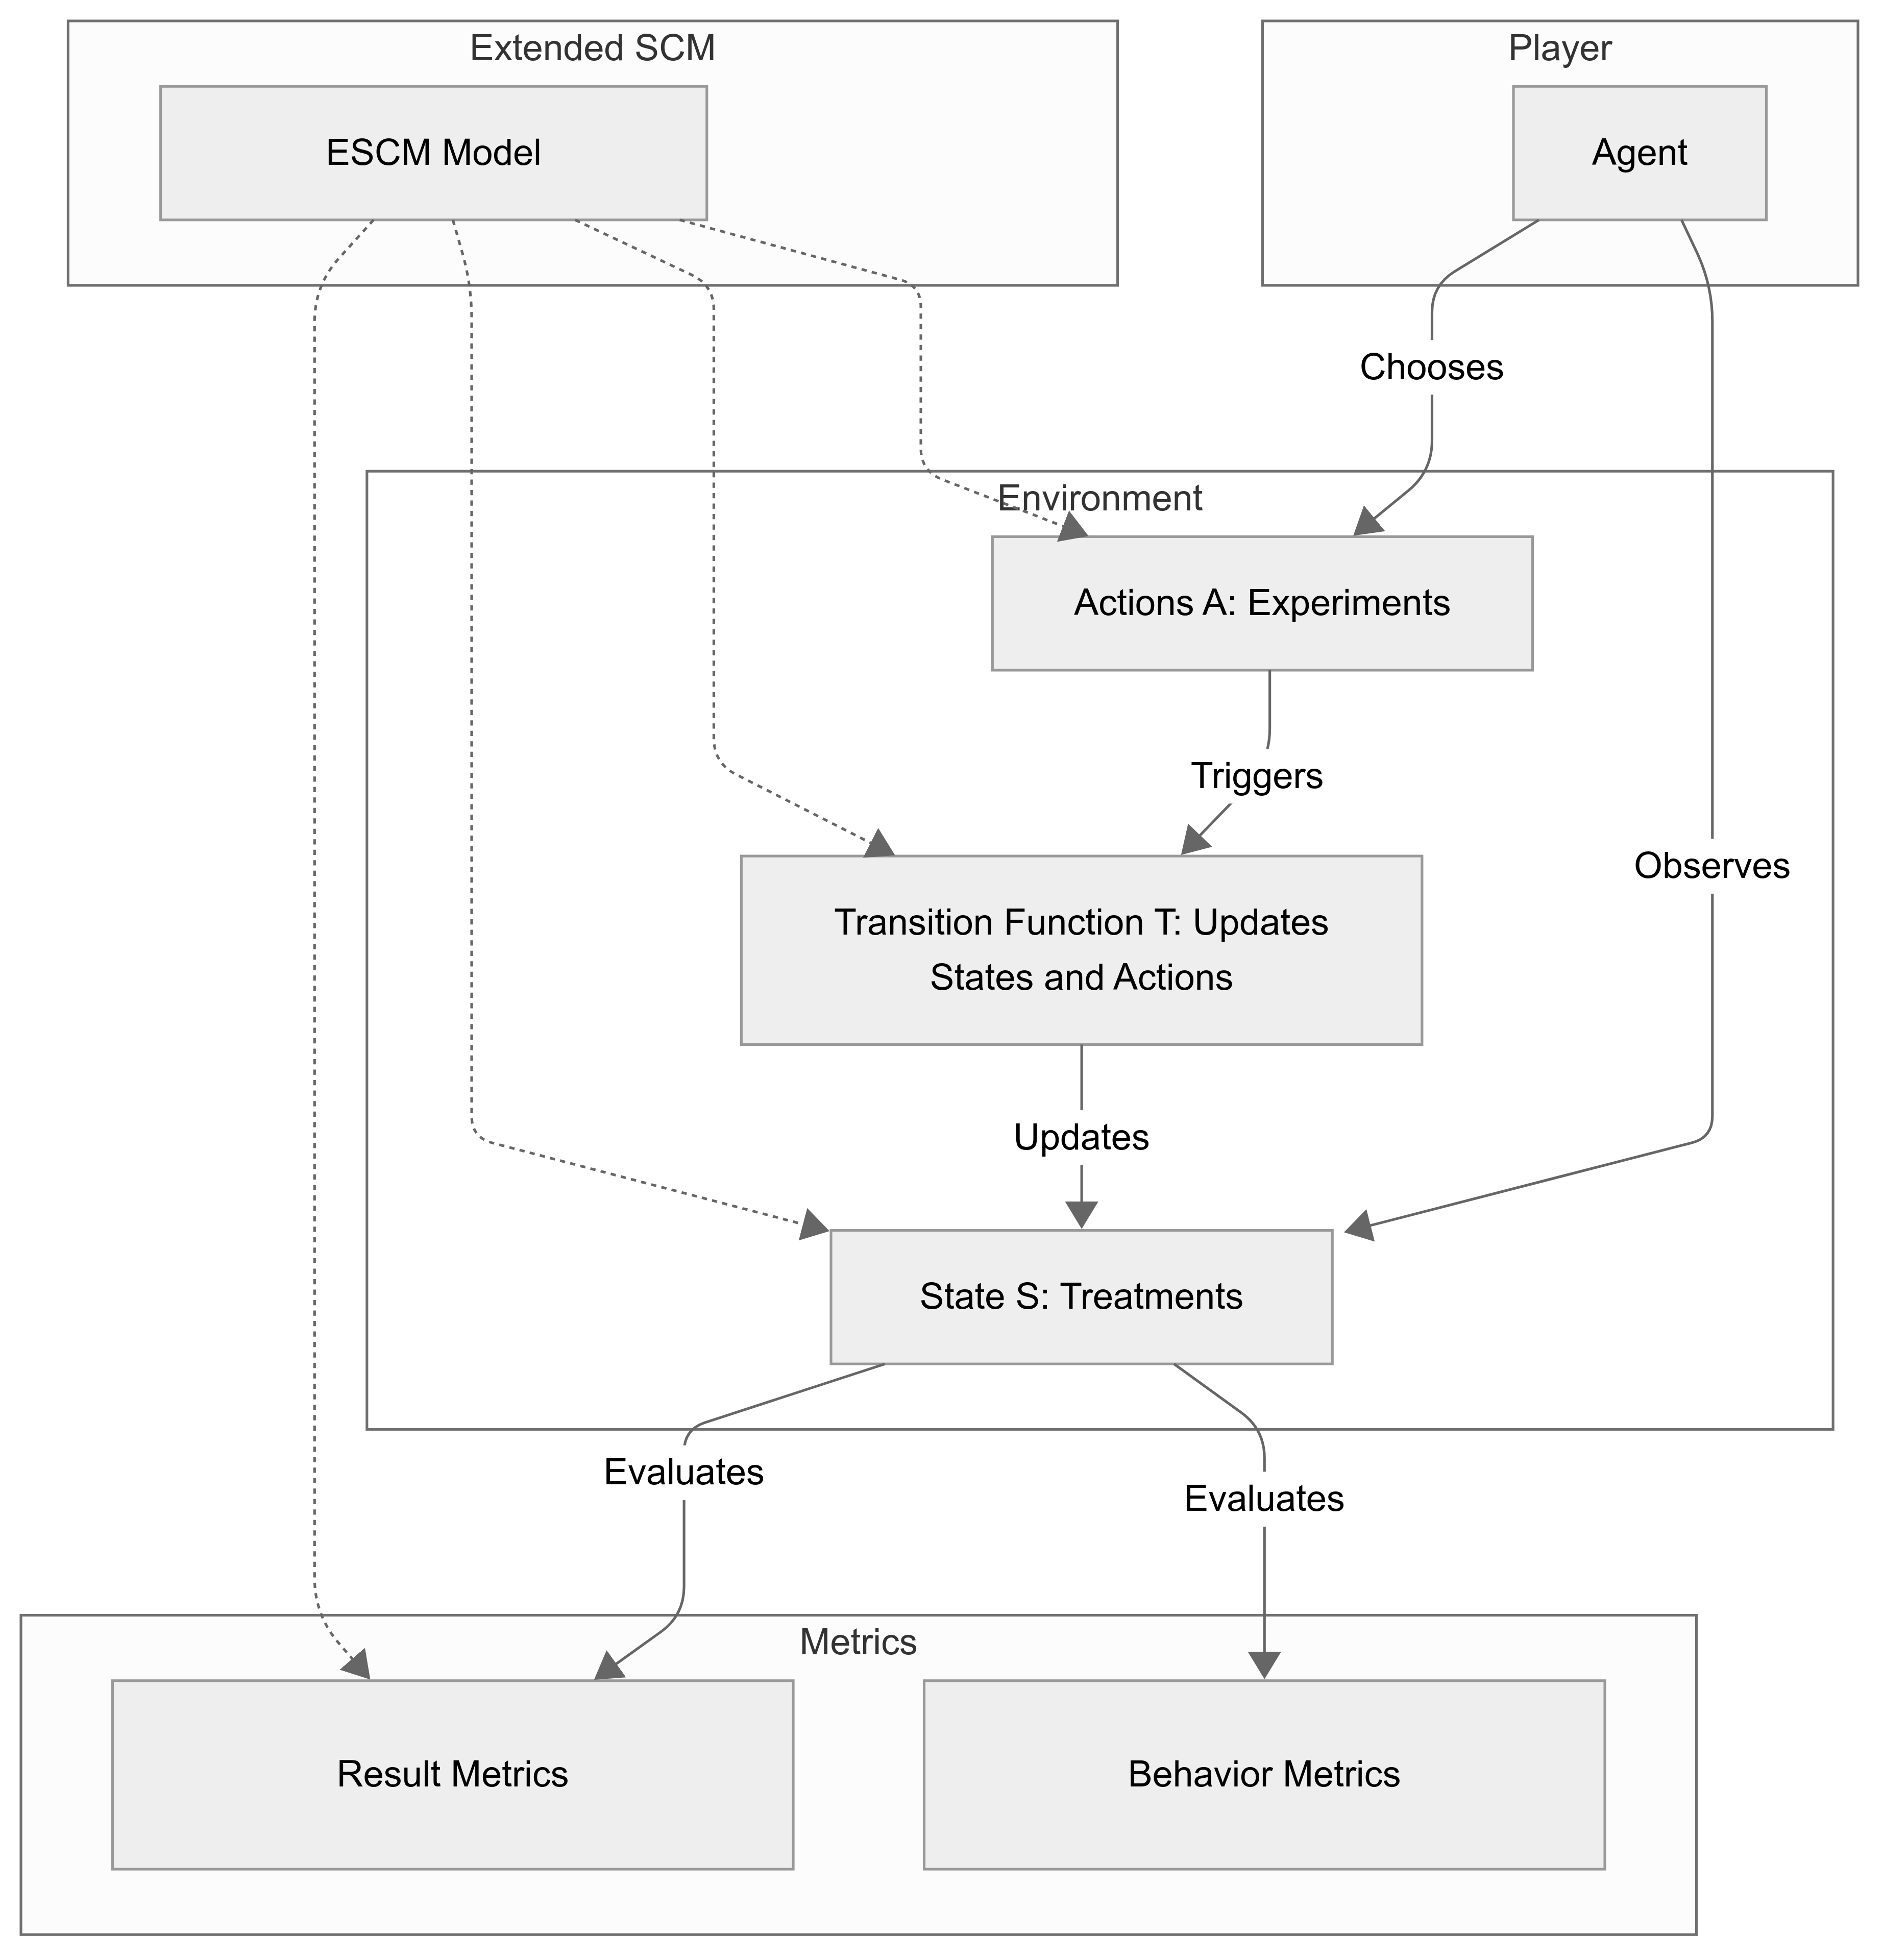
\includegraphics[width=0.7\columnwidth]{assets/game_components.png}
            \caption{
                % Diagram of \game components: the \textbf{State ($\statespace$)} captures treatments (\treatments), \textbf{Actions ($\actionspace$)} represent available experiments (\experiments) and responses, and the \textbf{Transition Function ($\transition$)} updates both the State ($\statespace$) and Actions ($\actionspace$) based on the agent's choices. 
                % Additionally the Player, the Extended Structural Causal Model ($\scm$) and the Performance Measure ($\performance$) are also shown.
                Game Components Diagram: The State ($\statespace$) captures treatments (\treatments), Actions ($\actionspace$) represent experiments (\experiments) and responses, and the Transition Function ($\transition$) updates both based on the agent’s choices. The diagram also includes the Player, the Extended Structural Causal Model ($\scm$), and the Performance Measure ($\performance$).
            } 
            \label{fig:game_components}
        \end{figure}



    \subsection{The Environment of a Match}
        The environment in \game serves as an interactive platform where causal discovery agents engage with a simulated world designed for experimentation. 
        It provides agents the capability to execute interventions and analyze the resulting datasets, facilitating the discovery of underlying causal structures. 
        While the environment leverages the extended SCM for implementing the dynamics of state transitions, it does not directly expose the SCM to the agent.
        This distinction emphasizes that the environment’s primary role is to enable agents to perform structured interventions and observe their outcomes while preventing direct access to the true causality.

        A single \emph{experiment} consists of defining how a collection of randomly sampled populations of subjects should be controlled in terms of the variables \varset.
        The set of \emph{treatments} $\treatments := \{t~|~t:X_i \rightarrow domain(X_i)~|~X_i \in \controllablex\}$ is the set of all assignments of variables to a possible value.
        Note that a treatment is a \emph{partial} mapping, i.e., does not need to assign a value to each variable; in particular, we denote as $\bot$ the \emph{empty treatment}, i.e., where \emph{no} variable has a value assigned.
        An experiment assigns to each treatment a number of subjects that should be observed with these (enforced) conditions, i.e., $\experiments := \{e~|~ e: \treatments \rightarrow \mathbb{N}\}$.


        The environment is then a tuple $\langle \statespace, \actionspace, \transition \rangle$ with the following syntax and semantics.
        The \emph{state space}, $\statespace$, comprises all possible states $s: \treatments \rightarrow \dataset$, each of them being a mapping between treatments and datasets with observations associated with these treatments. 
        The \emph{action space}, $\actionspace = \experiments \cup \{\text{stop with answer } a ~|~ a \in \outputspace\}$, encompasses all admissible interventions, where each action is either the execution of an experiment or stopping the game with a final answer.
        The state transition function $\transition$ encapsulates the dynamic evolution of the environment. 
        It maps a state-action pair $(s, a)$ to a subsequent state $s'$ depending on the nature of the action $a$.
        If $a$ is a regular experiment $\{(t_1, n_1),..,(t_k,n_k)\}$, then \transition samples a new dataset $D_i'$ of size $n_i$ for each treatment $t_i$, and we obtain $s'$ by first setting $s' := s$ and then sequentially updating $s' := (s' \setminus \{(t_i, D_i)\}) \cup \{(t_i, D_i \cup D_i')\}$ for all treatments $t_i$ in the experiment $a$, and where $D_i$ is the (maybe empty) dataset associated with treatment $t_i$ in the previous state $s$.
        If $a$ is a stopping action, then \transition transits to a distinguished final state $s^*$ that is equal to $s$ except that a final answer has been stored (here omitted from the formalization of \statespace to keep notation uncluttered), and no more actions are possible from $s^*$.
        


    \subsection{Initial State ($\initstate$)}
        The initial state $s_0$ may be any state from \statespace.
        Typically, it will contain only data for the empty treatment $\bot$ or even be entirely empty.



    \subsection{Stopping Condition $\phi$}
        Let \runs be the set of all possible alternating state-action sequences in the environment.
        The \emph{stopping condition} is a predicate $\phi$ that evaluates positively on a subset of \runs.
    
        There are two conditions that cause $\phi$ to evaluate positively on a run $r \in \runs$:

        \begin{enumerate}
            \item \textbf{Completion of Objectives:} Executing the stop action with an answer $a$.
            \item \textbf{Resource Limits:} A maximum number of actions or rounds as configured in the environment.
        \end{enumerate}



    \subsection{Performance Measure}
        The agent performance measure \performance is based on both the behavior \emph{during} the game (e.g., which and how many actions are necessary to achieve the goal), and the \emph{delivered solution} $o \in \outputspace$ (e.g., how similar is the identified causal model to SCM \scm).
        Formally, we define $\performance: \runs \rightarrow \mathbb{R}^2$, where the first component is based on the whole trajectory of the agent and the second is based only on the answer given in the last action (if any).



    \subsection{Match Simulation and Scoring}
        The simulation process begins by using a Structural Causal Model (SCM) to define the environment and evaluate a player’s strategy. 
        The system’s transition dynamics are derived from the SCM, and the simulation starts in an initial state $\initstate$. 
        The player iteratively selects actions, leading to state transitions until a stopping condition is met. 
        Throughout, the trajectory of states and actions is recorded and later assessed using performance metrics that evaluate both behavior and solution quality.

    The following Pseudocode presents the code implementation of this process.

        \begin{algorithm}
            \SetAlgoLined
            \KwIn{
                SCM $scm$ defining $\langle X, f_i, \eta \rangle$, \\
                Initial state $s_0$, \\
                Stopping condition $\phi(r)$, \\
                Performance measure $p(r)$, \\
                Player strategy $\pi(s)$
            }
            \KwOut{
                Run metrics $r = (\text{behavior}, \text{delivered})$
            }
            
            \SetKwFunction{GetEnvironment}{GetEnvironment}
            \SetKwFunction{GetAction}{GetAction}
            \SetKwFunction{UpdateState}{UpdateState}
            \SetKwFunction{ComputePerformance}{ComputePerformance}

            \tcp{Create the environment from SCM}
            $\langle \statespace, \actionspace, \transition \rangle \gets$ \GetEnvironment{$scm$} \\
            $s \gets s_0$ \tcp*{Initialize State} 
            $r \gets [s_0]$ \tcp*{Initialize Run}
            
            \While{\textbf{not} $\phi(r)$}{
                $a \gets \pi(s)$ \tcp*{Player's action}
                $s \gets \tau(s, a)$ \tcp*{Transition's State}
                $r.extend([a, s])$; \tcp*{Extend Run}
            }
            
            \Return{$p(r)$} \tcp*{Return Run Metrics}
            
            \caption{Run Match Simulation and Scoring with Post-Action Performance Calculation}
        \end{algorithm}







\section{Standard Components}
    To effectively being able to play \game with any player \texttt{pi}, one needs concrete realizations of \texttt{scm}, \texttt{s0}, \texttt{phi}, and the performance \texttt{p}.
    While the game (and our implementation) are open for any custom realizations of these components, we provide standard implementations to ease the usage.

        \begin{figure}[ht]
            \centering
            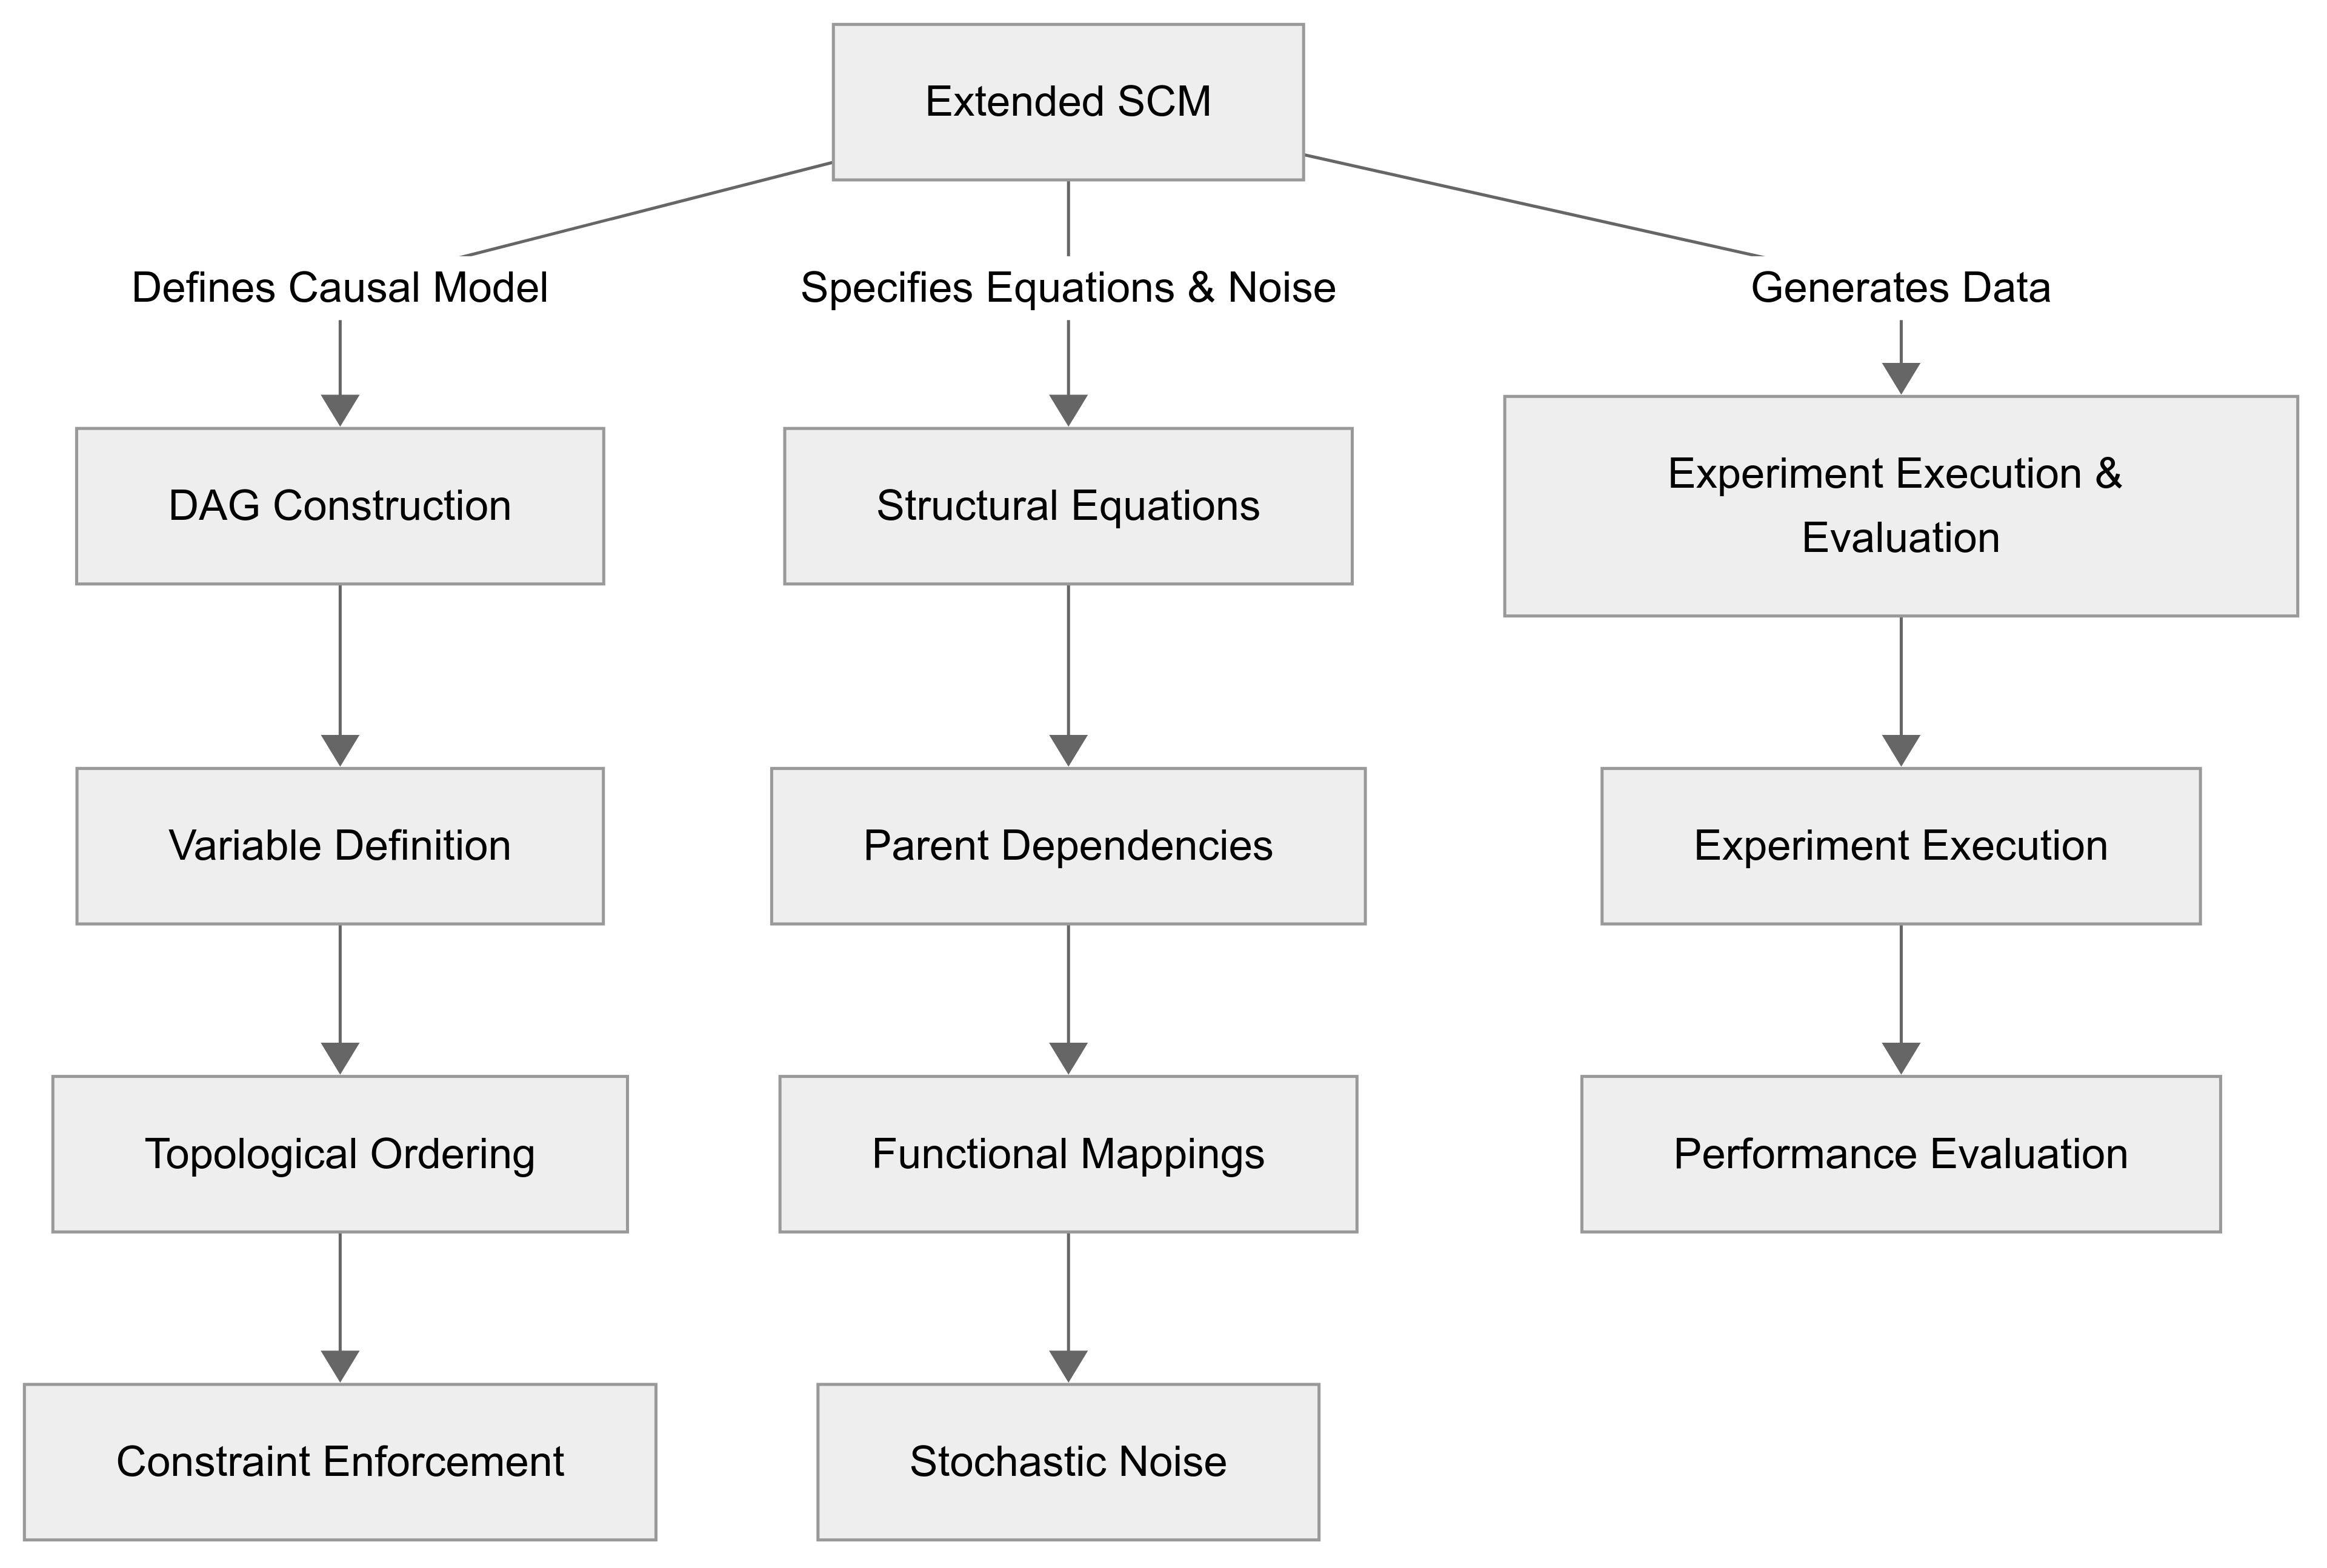
\includegraphics[width=0.7\columnwidth]{assets/scm_generation.png} % Replace with actual file path
            \caption{Diagram illustrating the Extended SCM process, capturing DAG construction, structural equations, and experiment execution.}
            \label{fig:scm_generation}
        \end{figure}



    \subsection{Standard SCM}
        The SCM serves as the foundation for generating experiments with interventional data and acts as the ground truth for evaluating agent performance. 
        The SCM is constructed systematically based on two primary components: 
        (1) the Directed Acyclic Graph (DAG) that defines the causal structure, and 
        (2) the equations and noise distributions that specify the causal relationships and stochastic behaviors of the variables.
        Both components are governed by hyperparameters that influence the nature of the SCM to be generated.
        We now discuss both components in detail.

        \begin{figure}[ht]
            \centering
            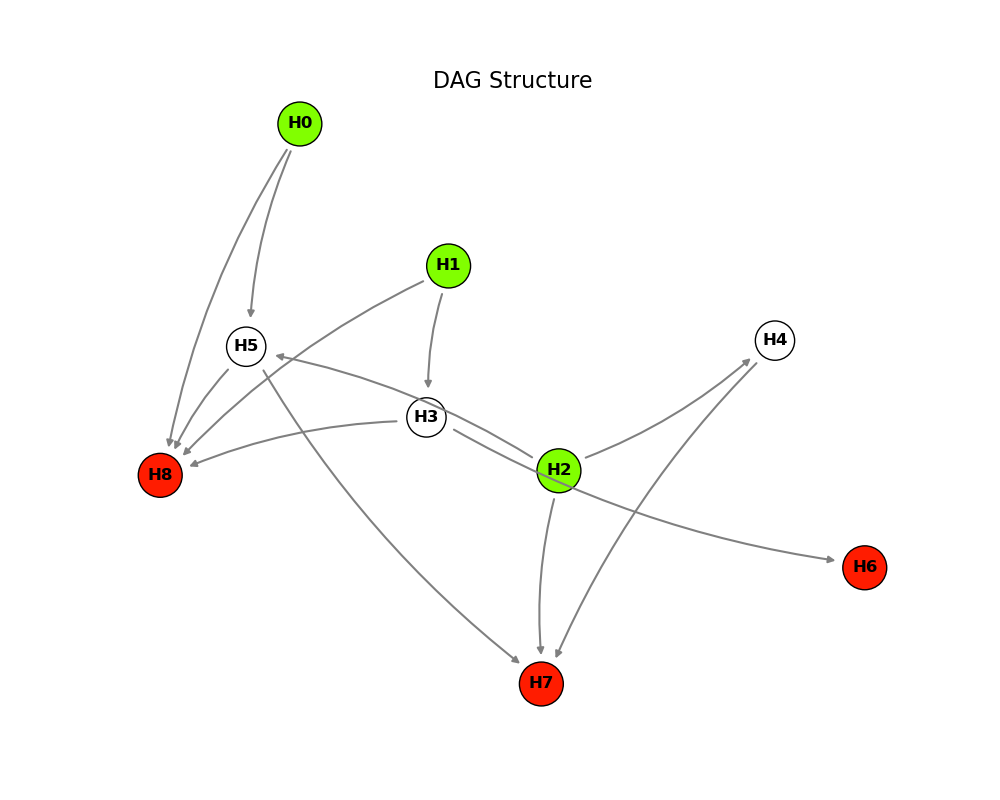
\includegraphics[width=0.7\columnwidth]{assets/dag_example.png} % Replace with actual file path
            \caption{An example of a Directed Acyclic Graph (DAG) used in \game. Root nodes ($\mathcal{R}$) are shown in green, intermediate nodes ($\mathcal{I}$) are shown in white, and leaf nodes ($\mathcal{L}$) are shown in red. The edges represent causal relationships between variables.}
            \label{fig:dag_example}
        \end{figure}



        \subsubsection{Directed Acyclic Graph (DAG) Construction}
            We present a structured approach for DAG generation that ensures compliance with user-defined constraints while maintaining flexibility for custom implementations. 
            The process consists of four key steps: (1) Variable Initialization, (2) Backbone DAG Construction, (3) Edge Refinement and Path Control, and (4) Validation and Finalization. 
            Given a set of variables $ \varset = \{\varname_1, \varname_2, \dots, \varname_n\} $ arranged in a topological order, the goal is to construct a DAG $ \mathcal{G} = (\varset, \mathcal{E}) $, where $ \mathcal{E} \subseteq \varset \times \varset $ represents causal dependencies \citep{pearl}. 
            
            % The first step partitions the variables into \emph{root nodes} $ \mathcal{R} $ (nodes with no incoming edges), \emph{leaf nodes} $ \mathcal{L} $ (nodes with no outgoing edges), and \emph{intermediate nodes} $ \mathcal{I} $, with user-defined quantities. 
            % % The backbone DAG is then constructed using a breadth-first search (BFS) algorithm, which prioritizes short-range connections to create a minimal spanning structure, ensuring that each intermediate node has a path from at least one root node to at least one leaf node. 
            % The backbone DAG is then constructed using a breadth-first search (BFS) algorithm, which ensures that each intermediate node is reachable from at least one root and has a path to at least one leaf, maintaining acyclicity. 
            % To refine the structure, additional edges are introduced based on a controlled probability distribution that determines edge presence while enforcing constraints on edge density, degree limits, and path lengths. 
            % % Edges are assigned only from \emph{lower-indexed nodes} to \emph{higher-indexed nodes} to preserve topological order. 
            % The probability of an edge between two nodes is influenced by their relative topological distance, favoring connections that enhance structural coherence without excessive shortcutting. 
            % % A depth-first search (DFS) algorithm selectively extends paths to ensure that the minimum path length requirement is met, prioritizing nodes with limited incoming edges. 
            % Path length constraints are enforced by inserting intermediate nodes where necessary and ensuring paths adhere to the defined range.
            % Conversely, to prevent excessively long paths, the longest paths are analyzed, and redundant intermediate nodes are removed or shortcut edges are introduced where appropriate, ensuring structural coherence. 
            % Finally, the DAG undergoes a validation process to confirm acyclicity, adherence to all constraints, and overall structural consistency, concluding with the generated graph shown in Fig.~\ref{fig:dag_example}.

            The first step partitions the variables into \emph{root nodes} $ \mathcal{R} $ (nodes with no incoming edges), \emph{leaf nodes} $ \mathcal{L} $ (nodes with no outgoing edges), and \emph{intermediate nodes} $ \mathcal{I} $, with user-defined quantities. 
            The backbone DAG is constructed using a breadth-first search (BFS) algorithm, ensuring each intermediate node is reachable from at least one root and connects to at least one leaf while preserving acyclicity. 
            To refine the structure, additional edges are introduced based on a controlled probability distribution that determines edge presence while enforcing constraints on edge density, degree limits, and path lengths. 
            Path length constraints are enforced by strategically inserting intermediate nodes, ensuring compliance with the specified range. 
            Conversely, to prevent excessively long paths, the longest paths are analyzed, and redundant intermediate nodes are removed or shortcut edges are selectively introduced to maintain topological integrity. 
            Finally, the DAG undergoes a validation process to confirm acyclicity, adherence to all constraints, and overall structural consistency, concluding with the generated graph shown in Fig.~\ref{fig:dag_example}.
            The complete DAG Generation Algorithm is detailed in appendix~\ref{appendix:dag_generation_algorithm}.
            %A basic implementation of the DAG generation algorithm is:
            \begin{algorithm}
                \DontPrintSemicolon
                \KwIn{Configuration parameters $\theta$}
                \KwOut{Directed Acyclic Graph (DAG)}
            
                \tcp{Step 1: Partition Nodes}
                $\mathcal{R}, \mathcal{I}, \mathcal{L} \leftarrow$ \texttt{DefineNodes}($\theta$) 
                % \tcp{Identify root, intermediate, and leaf nodes}
            
                \tcp{Step 2: Construct Backbone}
                $G \leftarrow \texttt{ConnectNodes}(\mathcal{R}, \mathcal{I}, \mathcal{L})$ 
                % \tcp{Ensure reachability while maintaining acyclicity}
            
                \tcp{Step 3: Add Edges Based on Constraints}
                $G \leftarrow \texttt{FillEdges}(G, \theta)$
                %  \tcp{Introduce edges based on probability, path lengths, and degree constraints}
            
                \Return $G$
                \caption{DAG Generation Algorithm}
            \end{algorithm}
            


        \subsubsection{Variable Properties}  
            Each variable $ \varname_i $ is characterized by its role and interactions within the graph.  
            It can be \emph{measured} ($ \varname_i \in \measuredx $) or \emph{latent} ($ \varname_i \notin \measuredx $), and either \emph{controllable} ($ \varname_i \in \controllablex $) or \emph{non-controllable} ($ \varname_i \notin \controllablex $), resulting in four possible categories.  
            The proportions of latent and measured variables are governed by $ \pl $, while treatability (controllability) is determined by $ \pt $.  
            
            Each variable is classified as either \emph{discrete} or \emph{continuous} based on a probabilistic model governed by $ \pc $, ensuring a structured distribution of variable types.  
            Continuous variables are sampled from a predefined bounded range for numerical stability.  
            For discrete variables, \emph{cardinality} $ |\text{dom}(\varname_i)| $ defines the number of possible values, assigned via a categorical distribution that favors commonly observed domain sizes (e.g., binary or low-cardinality categories).  



    \subsection{Structural Causal Equation Generation}
        The parent set of a variable $ \varname_i $ is denoted as $ \text{Pa}(\varname_i) = \{ \varname_j \mid (\varname_j \to \varname_i) \in \mathcal{E} \} $, representing the causal dependencies defined by the DAG structure. 
        Each variable is assigned a structural equation of the form:
        \begin{equation*}
            \varname_i = f_i(\text{Pa}(\varname_i)) + \eta_i
        \end{equation*}
        where $ f_i $ is a deterministic function constrained by user-defined rules, and $ \eta_i \sim \mathbb{P}_{\eta_i} $ is an exogenous noise term drawn from a user-specified distribution. 
        Structural equations are generated once and stored, ensuring reproducibility and computational efficiency in subsequent data generation processes. 
        Further details on the equation generation process are provided in Appendix~\ref{appendix:structural_equations_algorithm}.



        \subsubsection{Structural Equations}
            Under the assumption that both parent and child variables are numerical, the structural equation $f_i$ is constructed through a rigorous, iterative process based on a \textbf{context-free grammar (CFG)}. 
            The function $f_i$ is designed to capture causal dependencies by incorporating parent variables $\text{Pa}(\varname_i)$ as inputs. 
            The equation is iteratively built by selecting mathematical operations and functions from a predefined set, while strictly adhering to user-defined constraints. 
            These constraints regulate function complexity by imposing restrictions on \emph{linearity} (allowing or disallowing non-linear terms), \emph{exponentiation} (limiting variable or scalar exponents), and \emph{permitted mathematical operations} (e.g., product, logarithmic, exponential, trigonometric). Additionally, they define the \emph{maximum function complexity}, such as the highest polynomial degree or total number of terms.
            Based on these rules, the function $f_i$ is generated using a symbolic framework (e.g., \texttt{SymPy}), and all coefficients are precomputed as numeric values. 
            After $f_i$ is obtained, an exogenous noise term $\eta_i$, drawn from a user-defined probability distribution $\mathbb{P}_{\eta_i}$, is added to account for stochasticity and latent influences. 

            \paragraph{Categorical Nodes}
                For nodes representing categorical output variables, we create one formula with output values standardized between 0 and 1 for each possible category, and the idea is to assign the category with the highest score.
                At node initialization, for each possible category, a distinct CFG-generated function is created using the node’s input variables.
                The problem is that the output domains of these formulae are not comparable, and it is likely that some category scores will be consistently smaller than the scores of others.
                To overcome this limitation, scores are normalized as follows.
                We evaluate each of the functions on a set of 1000 initial samples for the input variables and compute the empirical cumulative density function (CDF).
                During the generation of new samples, each category-specific function is evaluated with the values of the parent variables, and its output is passed through the corresponding stored CDF.
                %The resulting probabilities indicate how well each function’s output matches its historical distribution. 
                The final categorical output is then selected as the category whose associated function yields the highest score according to its CDF; note that these do not sum up to 1 as in a softmax output.
        
            \paragraph{Categorical Parents}
                The previously described CFG-based function generation assumes that all parent variables are numerical. 
                In many real-world scenarios, however, a mix of numerical and categorical variables is common. 
                For numerical parent variables, their raw values are directly used as inputs to the structural equation. 
                For categorical parent variables, a fixed mapping is established at node initialization that assigns each category a random constant numerical value. 
                This is equivalent to a linear combination over constant values masked with 0-1-s stemming from a Bernoulli encoding.
                When generating a sample, the current categorical value of the parent variable is simply mapped to its corresponding numerical value using this pre-established mapping. 
                This numeric value is then used as the input for constructing the function \( f_i \). 

            
            


            \paragraph{Final Formulation}  
                The final structural equation for a numerical variable is expressed as
                \begin{equation*}
                    \varname_i = \max \left( \min \left( f_i(\text{Pa}(\varname_i)) + \eta_i, \varname_i^{\text{max}} \right), \varname_i^{\text{min}} \right),
                \end{equation*}
                where $\varname_i^{\text{min}}$ and $\varname_i^{\text{max}}$ denote the variable’s domain limits. For categorical variables, an inverse mapping function $g_i^{-1}$ is applied to the computed value:
                \begin{equation*}
                    \varname_i = g_i^{-1}\bigl(f_i(\text{Pa}(\varname_i)) + \eta_i\bigr).
                \end{equation*}
                This ensures that all variables, whether numerical or categorical, remain within their valid domains while preserving the specified causal relationships.
        
        \subsubsection{Data Generation}
            Once structural equations, categorical transformations, and mappings are stored, data generation proceeds in a topological order to ensure that dependencies are respected. 
            This process supports both observational and interventional regimes. 
            In observational data generation, variable values are sampled according to the precomputed functions and noise distributions. 
            In interventional data generation, the user can specify fixed values for selected variables; these interventions override the standard computations for the affected nodes, while the rest of the network is evaluated as usual. 
            For each new sample, the stored function $ f_i $ is retrieved along with any necessary CDF transformations for categorical parents. 
            The equation \( f_i(\text{Pa}(\varname_i)) + \eta_i \) is then evaluated, followed by categorical post-processing where applicable.



    \subsection{Standard Initial States}
        The initial state can either be empty or include a specific number of random observations without intervention. 
        The complexity of the SCM—defined by factors such as node count, latent variables, measurable variables, and network connectivity determines the initial state configuration. 
        High complexity models (e.g., with many latent variables, dense relationships, or sparse networks) result in 1–3 treated variables and 100–500 sample points. 
        Simpler models default to an empty state.



    \subsection{Standard Stopping Criteria}
        The stopping criteria determine when the agent ends the game by either (1) completing objectives through the stop action with an answer or (2) reaching resource limits, such as a maximum number of actions or rounds configured in the environment. 
        Resource usage and the finality of actions are analyzed to ensure a systematic conclusion of the game.



    \subsection{Performance Measure Generator}
        Both the Resources and Completion of objetives scores are measured by individually analyzing the actions taken to measure the performance in terms of number of steps and weight of each action .... and the run as a whole.
        The variables $\dots$.



    \subsection{Standard Goals and Metrics}
        Pre-defined sets of metrics for outputs (which then imply goals) and behavior
                
        \begin{itemize}
            \item \textbf{Reconstruct the SCM:} The agent must infer the underlying structural causal model.
            \item \textbf{Reconstruct the DAG:} The agent must infer the underlying causal structure encoded by the DAG $\DAG$.
            \item \textbf{Identify Direct Causes:} The agent must identify the underlying inducers for a specific variable.
            \item \textbf{Quantify Causal Strength:} The agent must estimate the causal strength of relationships between specific variables.
        \end{itemize}

        Note the complexity range of the goals, from simple identification tasks to more complex causal strength estimation. 
        In addition, an agent is restricted to play the game for no more than one goal type. 

        \sa{PENDING: References for each goal.}

        \begin{figure}[h]
            \centering
            % DAG Diagram without circles around "True DAG" and "Inferred DAG"
            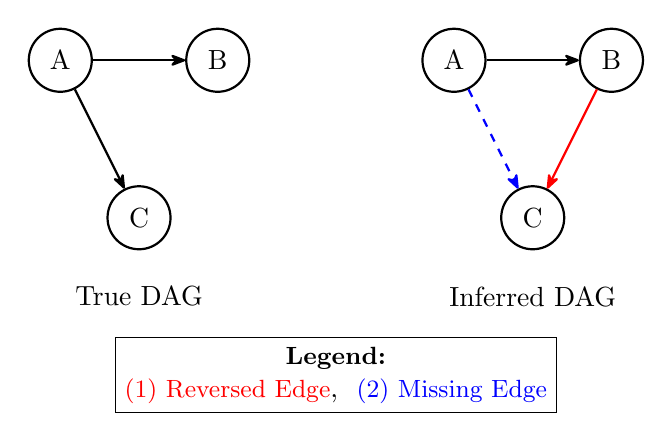
\begin{tikzpicture}[node distance=1.5cm and 2cm, >={Stealth[round]}, every node/.style={circle, draw, minimum size=0.8cm}]
                % True DAG
                \node[draw, thick] (T1) at (0,2) {A};
                \node[draw, thick] (T2) at (2,2) {B};
                \node[draw, thick] (T3) at (1,0) {C};
                
                \draw[->, thick] (T1) -- (T2);
                \draw[->, thick] (T1) -- (T3);
                
                \node[draw=none] at (1,-1) {True DAG}; % Remove the circle around this text
                
                % Inferred DAG
                \node[draw, thick] (I1) at (5,2) {A};
                \node[draw, thick] (I2) at (7,2) {B};
                \node[draw, thick] (I3) at (6,0) {C};
                
                \draw[->, thick] (I1) -- (I2);
                \draw[->, thick, red] (I2) -- (I3); % Reversal Error
                \draw[->, thick, blue, dashed] (I1) -- (I3); % Missing Edge
                
                \node[draw=none] at (6,-1) {Inferred DAG}; % Remove the circle around this text
                
                % Legend
                \node[rectangle, draw, align=center] at (3.5,-2){
                    \textbf{\small Legend:}\\
                    \textcolor{red}{\small(1) Reversed Edge}, \ 
                    \textcolor{blue}{\small(2) Missing Edge}
                };
            \end{tikzpicture}
            \caption{
                Comparison between the True DAG and Inferred DAG. 
                The true structure includes two edges originating from node A. 
                The inferred DAG introduces a reversed edge (red) and a missing edge (blue, dashed). 
            }
            \label{fig:true-inferred-dag}
        \end{figure}



        \subsubsection{Result Metrics}
            The following metrics are designed to assess the \emph{final answer} given by the agent.
            
            \paragraph{Uncover the SCM:}
                The \emph{Structural Hamming Distance (SHD)} evaluates discrepancies in the inferred DAG structure, while \emph{F1 Score} combines precision and recall for edge detection. 
                The \emph{Mean Squared Error (MSE)} quantifies deviations in the estimated functional relationships, and the \emph{Pearson Correlation Coefficient (PCC)} measures the alignment between the inferred and true causal strengths. 
                For counterfactual validation, the \emph{Average Treatment Effect (ATE)} assesses the accuracy of causal effect estimation.

            \paragraph{Reconstruct the DAG:}
                The \emph{Structural Hamming Distance (SHD)} quantifies discrepancies in edges between the inferred and the true DAG.
                The \emph{F1 Score} combines precision and recall for edge detection, while \emph{Edge Orientation Accuracy} evaluates the correctness of the causal direction.
            
            \paragraph{Identify Direct Causes:}
                \emph{Precision} measures the proportion of correctly identified direct causes, and \emph{Recall} captures how many true direct causes are found. 
                The \emph{F1 Score} balances these metrics, and \emph{Direct Causes Overlap} evaluates the similarity between the inferred and true direct causes.
            
            \paragraph{Quantify Causal Strength:}
                The \emph{Mean Absolute Error (MAE)} calculates deviations between inferred and true strengths. 
                \emph{Pearson Correlation Coefficient (PCC)} measures linear alignment, and \emph{Coverage Probability} checks if true values fall within confidence intervals.

            For instance, in Fig.~\ref{fig:true-inferred-dag}, the inferred DAG has discrepancies with the true DAG, such as a reversed edge (red) and a missing edge (blue, dashed).
            Which in the case of the goal \emph{DAG reconstruction} would lead to a high \emph{SHD} with low \emph{Edge Orientation Accuracy} and low \emph{F1} score.

            Beyond structural metrics, some measures, like \emph{ATE}, rely on assessing the causal effects encoded by the graph, which requires counterfactual reasoning to accurately evaluate these effects.

            \paragraph{Counterfactuals:}
                Counterfactual reasoning is fundamental to evaluating causal inference in \game. 
                Counterfactuals enable the benchmark to internally compute hypothetical outcomes of interventions, providing a robust foundation for result metrics. 
                A counterfactual under an intervention $\text{do}(\varname_i = v)$ is mathematically defined as:
                    \begin{equation*}
                        P(\varname_j \mid \text{do}(\varname_i = v)) = P(\varname_j \mid \text{Pa}(\varname_j) \setminus \varname_i = v),
                    \end{equation*}
                where $\varname_i$ is the intervened variable, $v$ is its fixed value, and $\varname_j$ represents the affected variable. 
                This captures how manipulating $\varname_i$ influences downstream outcomes through the causal structure.

                While agents do not compute counterfactuals directly, the benchmark uses counterfactual reasoning to evaluate agent performance. 

                For example, the Average Treatment Effect (ATE), a widely used causal effect measure, is calculated as:
                    \begin{equation*}
                        \text{ATE} = \mathbb{E}[Y \mid \text{do}(X = 1)] - \mathbb{E}[Y \mid \text{do}(X = 0)],
                    \end{equation*}
                where $X$ represents the treatment and $Y$ the outcome. 
                This quantifies the causal impact of an intervention on $ Y $ and serves as a reference for evaluating agent predictions.

                By leveraging counterfactuals internally, the benchmark rigorously assesses an agent's ability to infer causality using observational and interventional data. 



        \subsubsection{Behavior Metrics}
            The following metrics provide a detailed assessment of the agent’s \emph{behavior} and \emph{actions} throughout the game. 
            Once the game concludes, the agent's performance is evaluated based on the number of \emph{experiments}, \emph{treatments}, and \emph{rounds} executed. 
            Each action incurs a penalty, ensuring that efficient decision-making is rewarded.

            \paragraph{Penalty Measures}
                The penalties for experiments, treatments, and rounds are defined as weighted costs:
                \begin{equation*}
                    \penalties_{\experiments} = e \cdot n_\experiments, \quad
                    \penalties_{\treatments} = t \cdot n_\treatments, \quad
                    \penalties_{\runs} = r \cdot n_\runs.
                \end{equation*}
                where $ n_\experiments $, $ n_\treatments $, and $ n_\runs $ represent the total number of \emph{experiments}, \emph{treatments}, and \emph{rounds}, respectively, and $ e, t, r $ are their associated cost coefficients.


            \paragraph{Total Behaviour Measure:}
                The total behavior measure is the weighted average of the penalties incurred by the agent during the game:
                    \begin{equation*}
                        \penalties_{\text{total}} = \alpha \cdot \penalties_{\experiments} + \beta \cdot \penalties_{\treatments} + \gamma \cdot \penalties_{\runs}.
                    \end{equation*}
                where $\alpha$, $\beta$, and $\gamma$ are the weights assigned to each penalty, ensuring a balanced evaluation of the agent's behavior.

                
            \paragraph{Monotonicity Property}
                This function is \emph{monotonic} over the set of all possible game histories, meaning that increasing the number of experiments, treatments, or rounds strictly increases the penalty. 
                Formally, if $\runs$ and $\runs'$ are two game histories such that:
                \begin{equation*}
                    n_\experiments \geq n_\experiments, \quad
                    n_\treatments \geq n_\treatments, \quad
                    n_\runs' \geq n_\runs,
                \end{equation*}
                then:
                \begin{equation*}
                    \penalties_{\text{total}}(\runs') \geq \penalties_{\text{total}}(\runs).
                \end{equation*}
                This guarantees that the behavior measure respects efficiency, discouraging unnecessary actions while rewarding optimal strategies.


        \subsubsection{Combined Final Metric}
            To comprehensively evaluate an agent, a global measure integrates the \emph{result metrics} (task performance) and \emph{behavior metrics} (efficiency and costs). This ensures a balanced assessment of both solution quality and execution efficiency.
            
            \paragraph{Result Metrics Aggregate}  
                The result metrics are normalized to $[0,1]$ and combined into a single score:
                \begin{equation*}
                    \mathcal{M}_{\text{result}} = w_1 \cdot \text{SHD}_{\text{norm}} + w_2 \cdot \text{F1} + w_3 \cdot \text{MSE}_{\text{norm}} + w_4 \cdot \text{PCC},
                \end{equation*}
                where $ w_1, w_2, w_3, w_4 $ control the relative importance of each component.
            
            \paragraph{Behavior Metrics Aggregate}  
                The behavior score accounts for the penalties incurred from agent actions:
                \begin{equation*}
                    \mathcal{M}_{\text{behavior}} = \alpha \cdot \penalties_{\experiments} + \beta \cdot \penalties_{\treatments} + \gamma \cdot \penalties_{\runs},
                \end{equation*}
                where $\penalties_{\experiments}$, $\penalties_{\treatments}$, and $\penalties_{\runs}$ represent penalties for the number of experiments, treatments, and rounds, respectively, where $ \alpha, \beta, \gamma $ adjust for different cost contributions.
            
            \paragraph{Global Measure}  
                The final evaluation metric combines both aspects:
                \begin{equation*}
                    \mathcal{M}_{\text{global}} = \lambda \cdot \mathcal{M}_{\text{result}} + (1 - \lambda) \cdot \mathcal{M}_{\text{behavior}},
                \end{equation*}
                where $ \lambda \in [0,1] $ controls the trade-off between result quality and efficiency. The global measure ranges from 0 (poor performance) to 1 (optimal performance), ensuring interpretability.







\section{Results}
  Results







\section{Discussion}
  Discussion







\section{Conclusion}
  Conclusion










  \appendix

  \section{DAG Generation Algorithm}
      \label{appendix:dag_generation_algorithm}
      \begin{algorithm}
          \caption{Optimized Directed Acyclic Graph (DAG) Generation}
          \KwIn{Number of nodes $N$, number of roots $R$, number of leaves $L$, edge density $D$, max in-degree $M_{\text{in}}$, max out-degree $M_{\text{out}}$, min/max path lengths $P_{\text{min}}, P_{\text{max}}$}
          \KwOut{A valid DAG $ \mathcal{G} = (\varset, \mathcal{E}) $}
          
          \BlankLine
          \textbf{Step 1: Initialize Nodes and Partitions} \\
          Partition $ \varset $ into:
          \begin{itemize}
              \item Root nodes $ \mathcal{R} $ (no incoming edges)
              \item Leaf nodes $ \mathcal{L} $ (no outgoing edges)
              \item Intermediate nodes $ \mathcal{I} = \varset \setminus (\mathcal{R} \cup \mathcal{L}) $
          \end{itemize}
          
          \BlankLine
          \textbf{Step 2: Construct Backbone DAG (BFS-based)} \\
          Initialize $ \mathcal{G} = (\varset, \emptyset) $ \;
          \ForEach{node $ v \in \varset $}{
              Add $ v $ to $ \mathcal{G} $
          }
          \ForEach{root node $ r \in \mathcal{R} $}{
              Perform BFS from $ r $ to establish at least one path from $ r $ to $ l \in \mathcal{L} $ \;
              Ensure each intermediate $ i \in \mathcal{I} $ has at least one incoming and one outgoing edge
          }
          
          \BlankLine
          \textbf{Step 3: Edge Refinement and Constraints} \\
          Compute valid edge pairs: \;
          \ForEach{pair $ (i, j) $ where $ i < j $}{
              \If{$ i \notin \mathcal{L} $ and $ j \notin \mathcal{R} $ and $ (i, j) \notin (\mathcal{R} \times \mathcal{R}) $}{
                  Add edge $ (i, j) $ with probability $ P(i,j) \leq D $, where $ P(i,j) \sim U(0,1) $.
              }
          }
          
          \BlankLine
          \textbf{Step 4: Path Length Adjustment (Precomputed Shortest Paths)} \\
          Compute all paths for all node pairs in $ \mathcal{G} $\;
          \ForEach{pair $ (r, l) $ where $ r \in \mathcal{R}, l \in \mathcal{L} $}{
              \If{path length $ P(r, l) < P_{\text{min}} $}{
                  Insert an intermediate node to extend the path
              }
              \If{path length $ P(r, l) > P_{\text{max}} $}{
                  Introduce a shortcut edge to shorten the path
              }
          }
          
          \BlankLine
          \textbf{Step 5: Validation and Finalization} \\
          \If{$\mathcal{G}$ contains cycles}{
              Remove edges iteratively until acyclicity is restored
          }
  
          \Return{$\mathcal{G}$}
      \end{algorithm}
  
  \section{Structural Equations Algorithm for SCM's}
      \label{appendix:structural_equations_algorithm}
      \begin{algorithm}
          \DontPrintSemicolon
          \SetKwInput{Input}{Input}
          \SetKwInput{Output}{Output}
          \SetKwFunction{GenerateFunction}{GenerateFunction}
          \SetKwFunction{ComputeCDF}{ComputeCDF}
          \SetKwFunction{OneHotEncode}{OneHotEncode}
          \SetKwFunction{SelectCategory}{SelectCategory}
          \SetKwFunction{StoreMapping}{StoreMapping}
          
          \Input{
              DAG $ \mathcal{D} = (\mathcal{X}, \mathcal{E}) $;\\
              Variable types $ \mathcal{T} = \{T_i\} $ (numerical or categorical);\\
              User constraints on function generation;\\
              Predefined variable domains.
          }
          \Output{
              Stored structural equations $ \mathcal{F} = \{ f_i \} $,\\
              CDFs for categorical transformations $ \mathcal{G} = \{ g_j \} $,\\
              Stored categorical mappings $ \mathcal{M} $.
          }
          
          \BlankLine
          \textbf{One-Time Structural Equation and Transformation Generation:} \\
          
          \ForEach{variable $ \varname_i \in \mathcal{X} $ in topological order}{
              \If{$ \varname_i $ is a root node}{
                  $ f_i \gets $ Exogenous distribution $ \mathbb{P}_{\varname_i} $ \;
                  Store $ f_i $ in $ \mathcal{F} $ \;
               %  \Continue
                  \textbf{continue}\; 
              }
              
              Identify parent set $ \text{Pa}(\varname_i) $ from $ \mathcal{D} $ \;
              
              \BlankLine
              \textbf{Handle Parent Variables:} \\
              \ForEach{$ \varname_j \in \text{Pa}(\varname_i) $}{
                  \If{$ \varname_j $ is categorical}{
                      One-hot encode $ \varname_j $ into binary variables $ \{ B_{j1}, B_{j2}, ..., B_{jk} \} $ \;
                      \ForEach{binary variable $ B_{jm} $}{
                          Generate function $ g_{jm} \gets \GenerateFunction(\text{user constraints}) $ \;
                          Compute CDF $ \mathcal{G}[B_{jm}] \gets \ComputeCDF(g_{jm}) $ \;
                          Store $ g_{jm} $ and $ \mathcal{G}[B_{jm}] $ \;
                      }
                  }
              }
              
              \BlankLine
              \textbf{Generate Structural Equation:} \\
              Define input variables:
              $ V_i \gets $ numerical parents $ + $ transformed categorical parents \;
              Generate function $ f_i \gets \GenerateFunction(V_i, \text{user constraints}) $ \;
              Store $ f_i $ in $ \mathcal{F} $ \;
              
              \BlankLine
              \textbf{Store Categorical Output Mapping (if needed):} \\
              \If{$ \varname_i $ is categorical}{
                  Assign random numerical values to each category \;
                  Store category mapping in $ \mathcal{M}[\varname_i] $ \;
              }
          }
  
          \Return{$ \mathcal{F} $, $ \mathcal{G} $, $ \mathcal{M} $}
          
          \BlankLine
          \textbf{Data Generation Using Stored Equations:} \\
          
          \ForEach{variable $ \varname_i \in \mathcal{X} $}{
              Retrieve stored function $ f_i $ \;
              Retrieve stored CDFs for categorical parents, if applicable \;
              
              \If{$ \varname_i $ is numerical}{
                  Compute $ \varname_i \gets f_i(\text{Pa}(\varname_i)) + \eta_i $ \;
              }
              \ElseIf{$ \varname_i $ is categorical}{
                  Compute output value $ z \gets f_i(\text{Pa}(\varname_i)) + \eta_i $ \;
                  Assign category $ \varname_i \gets \SelectCategory(z, \mathcal{M}[\varname_i]) $ \;
              }
          }
          
          \caption{Structural Causal Equation Generation}
      \end{algorithm}















\newpage
\section*{NeurIPS Paper Checklist}

%%% BEGIN INSTRUCTIONS %%%
The checklist is designed to encourage best practices for responsible machine learning research, addressing issues of reproducibility, transparency, research ethics, and societal impact. Do not remove the checklist: {\bf The papers not including the checklist will be desk rejected.} The checklist should follow the references and follow the (optional) supplemental material.  The checklist does NOT count towards the page
limit. 

Please read the checklist guidelines carefully for information on how to answer these questions. For each question in the checklist:
\begin{itemize}
    \item You should answer \answerYes{}, \answerNo{}, or \answerNA{}.
    \item \answerNA{} means either that the question is Not Applicable for that particular paper or the relevant information is Not Available.
    \item Please provide a short (1–2 sentence) justification right after your answer (even for NA). 
   % \item {\bf The papers not including the checklist will be desk rejected.}
\end{itemize}

{\bf The checklist answers are an integral part of your paper submission.} They are visible to the reviewers, area chairs, senior area chairs, and ethics reviewers. You will be asked to also include it (after eventual revisions) with the final version of your paper, and its final version will be published with the paper.

The reviewers of your paper will be asked to use the checklist as one of the factors in their evaluation. While "\answerYes{}" is generally preferable to "\answerNo{}", it is perfectly acceptable to answer "\answerNo{}" provided a proper justification is given (e.g., "error bars are not reported because it would be too computationally expensive" or "we were unable to find the license for the dataset we used"). In general, answering "\answerNo{}" or "\answerNA{}" is not grounds for rejection. While the questions are phrased in a binary way, we acknowledge that the true answer is often more nuanced, so please just use your best judgment and write a justification to elaborate. All supporting evidence can appear either in the main paper or the supplemental material, provided in appendix. If you answer \answerYes{} to a question, in the justification please point to the section(s) where related material for the question can be found.

IMPORTANT, please:
\begin{itemize}
    \item {\bf Delete this instruction block, but keep the section heading ``NeurIPS Paper Checklist"},
    \item  {\bf Keep the checklist subsection headings, questions/answers and guidelines below.}
    \item {\bf Do not modify the questions and only use the provided macros for your answers}.
\end{itemize} 
 

%%% END INSTRUCTIONS %%%


\begin{enumerate}

\item {\bf Claims}
    \item[] Question: Do the main claims made in the abstract and introduction accurately reflect the paper's contributions and scope?
    \item[] Answer: \answerTODO{} % Replace by \answerYes{}, \answerNo{}, or \answerNA{}.
    \item[] Justification: \justificationTODO{}
    \item[] Guidelines:
    \begin{itemize}
        \item The answer NA means that the abstract and introduction do not include the claims made in the paper.
        \item The abstract and/or introduction should clearly state the claims made, including the contributions made in the paper and important assumptions and limitations. A No or NA answer to this question will not be perceived well by the reviewers. 
        \item The claims made should match theoretical and experimental results, and reflect how much the results can be expected to generalize to other settings. 
        \item It is fine to include aspirational goals as motivation as long as it is clear that these goals are not attained by the paper. 
    \end{itemize}

\item {\bf Limitations}
    \item[] Question: Does the paper discuss the limitations of the work performed by the authors?
    \item[] Answer: \answerTODO{} % Replace by \answerYes{}, \answerNo{}, or \answerNA{}.
    \item[] Justification: \justificationTODO{}
    \item[] Guidelines:
    \begin{itemize}
        \item The answer NA means that the paper has no limitation while the answer No means that the paper has limitations, but those are not discussed in the paper. 
        \item The authors are encouraged to create a separate "Limitations" section in their paper.
        \item The paper should point out any strong assumptions and how robust the results are to violations of these assumptions (e.g., independence assumptions, noiseless settings, model well-specification, asymptotic approximations only holding locally). The authors should reflect on how these assumptions might be violated in practice and what the implications would be.
        \item The authors should reflect on the scope of the claims made, e.g., if the approach was only tested on a few datasets or with a few runs. In general, empirical results often depend on implicit assumptions, which should be articulated.
        \item The authors should reflect on the factors that influence the performance of the approach. For example, a facial recognition algorithm may perform poorly when image resolution is low or images are taken in low lighting. Or a speech-to-text system might not be used reliably to provide closed captions for online lectures because it fails to handle technical jargon.
        \item The authors should discuss the computational efficiency of the proposed algorithms and how they scale with dataset size.
        \item If applicable, the authors should discuss possible limitations of their approach to address problems of privacy and fairness.
        \item While the authors might fear that complete honesty about limitations might be used by reviewers as grounds for rejection, a worse outcome might be that reviewers discover limitations that aren't acknowledged in the paper. The authors should use their best judgment and recognize that individual actions in favor of transparency play an important role in developing norms that preserve the integrity of the community. Reviewers will be specifically instructed to not penalize honesty concerning limitations.
    \end{itemize}

\item {\bf Theory assumptions and proofs}
    \item[] Question: For each theoretical result, does the paper provide the full set of assumptions and a complete (and correct) proof?
    \item[] Answer: \answerTODO{} % Replace by \answerYes{}, \answerNo{}, or \answerNA{}.
    \item[] Justification: \justificationTODO{}
    \item[] Guidelines:
    \begin{itemize}
        \item The answer NA means that the paper does not include theoretical results. 
        \item All the theorems, formulas, and proofs in the paper should be numbered and cross-referenced.
        \item All assumptions should be clearly stated or referenced in the statement of any theorems.
        \item The proofs can either appear in the main paper or the supplemental material, but if they appear in the supplemental material, the authors are encouraged to provide a short proof sketch to provide intuition. 
        \item Inversely, any informal proof provided in the core of the paper should be complemented by formal proofs provided in appendix or supplemental material.
        \item Theorems and Lemmas that the proof relies upon should be properly referenced. 
    \end{itemize}

    \item {\bf Experimental result reproducibility}
    \item[] Question: Does the paper fully disclose all the information needed to reproduce the main experimental results of the paper to the extent that it affects the main claims and/or conclusions of the paper (regardless of whether the code and data are provided or not)?
    \item[] Answer: \answerTODO{} % Replace by \answerYes{}, \answerNo{}, or \answerNA{}.
    \item[] Justification: \justificationTODO{}
    \item[] Guidelines:
    \begin{itemize}
        \item The answer NA means that the paper does not include experiments.
        \item If the paper includes experiments, a No answer to this question will not be perceived well by the reviewers: Making the paper reproducible is important, regardless of whether the code and data are provided or not.
        \item If the contribution is a dataset and/or model, the authors should describe the steps taken to make their results reproducible or verifiable. 
        \item Depending on the contribution, reproducibility can be accomplished in various ways. For example, if the contribution is a novel architecture, describing the architecture fully might suffice, or if the contribution is a specific model and empirical evaluation, it may be necessary to either make it possible for others to replicate the model with the same dataset, or provide access to the model. In general. releasing code and data is often one good way to accomplish this, but reproducibility can also be provided via detailed instructions for how to replicate the results, access to a hosted model (e.g., in the case of a large language model), releasing of a model checkpoint, or other means that are appropriate to the research performed.
        \item While NeurIPS does not require releasing code, the conference does require all submissions to provide some reasonable avenue for reproducibility, which may depend on the nature of the contribution. For example
        \begin{enumerate}
            \item If the contribution is primarily a new algorithm, the paper should make it clear how to reproduce that algorithm.
            \item If the contribution is primarily a new model architecture, the paper should describe the architecture clearly and fully.
            \item If the contribution is a new model (e.g., a large language model), then there should either be a way to access this model for reproducing the results or a way to reproduce the model (e.g., with an open-source dataset or instructions for how to construct the dataset).
            \item We recognize that reproducibility may be tricky in some cases, in which case authors are welcome to describe the particular way they provide for reproducibility. In the case of closed-source models, it may be that access to the model is limited in some way (e.g., to registered users), but it should be possible for other researchers to have some path to reproducing or verifying the results.
        \end{enumerate}
    \end{itemize}


\item {\bf Open access to data and code}
    \item[] Question: Does the paper provide open access to the data and code, with sufficient instructions to faithfully reproduce the main experimental results, as described in supplemental material?
    \item[] Answer: \answerTODO{} % Replace by \answerYes{}, \answerNo{}, or \answerNA{}.
    \item[] Justification: \justificationTODO{}
    \item[] Guidelines:
    \begin{itemize}
        \item The answer NA means that paper does not include experiments requiring code.
        \item Please see the NeurIPS code and data submission guidelines (\url{https://nips.cc/public/guides/CodeSubmissionPolicy}) for more details.
        \item While we encourage the release of code and data, we understand that this might not be possible, so “No” is an acceptable answer. Papers cannot be rejected simply for not including code, unless this is central to the contribution (e.g., for a new open-source benchmark).
        \item The instructions should contain the exact command and environment needed to run to reproduce the results. See the NeurIPS code and data submission guidelines (\url{https://nips.cc/public/guides/CodeSubmissionPolicy}) for more details.
        \item The authors should provide instructions on data access and preparation, including how to access the raw data, preprocessed data, intermediate data, and generated data, etc.
        \item The authors should provide scripts to reproduce all experimental results for the new proposed method and baselines. If only a subset of experiments are reproducible, they should state which ones are omitted from the script and why.
        \item At submission time, to preserve anonymity, the authors should release anonymized versions (if applicable).
        \item Providing as much information as possible in supplemental material (appended to the paper) is recommended, but including URLs to data and code is permitted.
    \end{itemize}


\item {\bf Experimental setting/details}
    \item[] Question: Does the paper specify all the training and test details (e.g., data splits, hyperparameters, how they were chosen, type of optimizer, etc.) necessary to understand the results?
    \item[] Answer: \answerTODO{} % Replace by \answerYes{}, \answerNo{}, or \answerNA{}.
    \item[] Justification: \justificationTODO{}
    \item[] Guidelines:
    \begin{itemize}
        \item The answer NA means that the paper does not include experiments.
        \item The experimental setting should be presented in the core of the paper to a level of detail that is necessary to appreciate the results and make sense of them.
        \item The full details can be provided either with the code, in appendix, or as supplemental material.
    \end{itemize}

\item {\bf Experiment statistical significance}
    \item[] Question: Does the paper report error bars suitably and correctly defined or other appropriate information about the statistical significance of the experiments?
    \item[] Answer: \answerTODO{} % Replace by \answerYes{}, \answerNo{}, or \answerNA{}.
    \item[] Justification: \justificationTODO{}
    \item[] Guidelines:
    \begin{itemize}
        \item The answer NA means that the paper does not include experiments.
        \item The authors should answer "Yes" if the results are accompanied by error bars, confidence intervals, or statistical significance tests, at least for the experiments that support the main claims of the paper.
        \item The factors of variability that the error bars are capturing should be clearly stated (for example, train/test split, initialization, random drawing of some parameter, or overall run with given experimental conditions).
        \item The method for calculating the error bars should be explained (closed form formula, call to a library function, bootstrap, etc.)
        \item The assumptions made should be given (e.g., Normally distributed errors).
        \item It should be clear whether the error bar is the standard deviation or the standard error of the mean.
        \item It is OK to report 1-sigma error bars, but one should state it. The authors should preferably report a 2-sigma error bar than state that they have a 96\% CI, if the hypothesis of Normality of errors is not verified.
        \item For asymmetric distributions, the authors should be careful not to show in tables or figures symmetric error bars that would yield results that are out of range (e.g. negative error rates).
        \item If error bars are reported in tables or plots, The authors should explain in the text how they were calculated and reference the corresponding figures or tables in the text.
    \end{itemize}

\item {\bf Experiments compute resources}
    \item[] Question: For each experiment, does the paper provide sufficient information on the computer resources (type of compute workers, memory, time of execution) needed to reproduce the experiments?
    \item[] Answer: \answerTODO{} % Replace by \answerYes{}, \answerNo{}, or \answerNA{}.
    \item[] Justification: \justificationTODO{}
    \item[] Guidelines:
    \begin{itemize}
        \item The answer NA means that the paper does not include experiments.
        \item The paper should indicate the type of compute workers CPU or GPU, internal cluster, or cloud provider, including relevant memory and storage.
        \item The paper should provide the amount of compute required for each of the individual experimental runs as well as estimate the total compute. 
        \item The paper should disclose whether the full research project required more compute than the experiments reported in the paper (e.g., preliminary or failed experiments that didn't make it into the paper). 
    \end{itemize}
    
\item {\bf Code of ethics}
    \item[] Question: Does the research conducted in the paper conform, in every respect, with the NeurIPS Code of Ethics \url{https://neurips.cc/public/EthicsGuidelines}?
    \item[] Answer: \answerTODO{} % Replace by \answerYes{}, \answerNo{}, or \answerNA{}.
    \item[] Justification: \justificationTODO{}
    \item[] Guidelines:
    \begin{itemize}
        \item The answer NA means that the authors have not reviewed the NeurIPS Code of Ethics.
        \item If the authors answer No, they should explain the special circumstances that require a deviation from the Code of Ethics.
        \item The authors should make sure to preserve anonymity (e.g., if there is a special consideration due to laws or regulations in their jurisdiction).
    \end{itemize}


\item {\bf Broader impacts}
    \item[] Question: Does the paper discuss both potential positive societal impacts and negative societal impacts of the work performed?
    \item[] Answer: \answerTODO{} % Replace by \answerYes{}, \answerNo{}, or \answerNA{}.
    \item[] Justification: \justificationTODO{}
    \item[] Guidelines:
    \begin{itemize}
        \item The answer NA means that there is no societal impact of the work performed.
        \item If the authors answer NA or No, they should explain why their work has no societal impact or why the paper does not address societal impact.
        \item Examples of negative societal impacts include potential malicious or unintended uses (e.g., disinformation, generating fake profiles, surveillance), fairness considerations (e.g., deployment of technologies that could make decisions that unfairly impact specific groups), privacy considerations, and security considerations.
        \item The conference expects that many papers will be foundational research and not tied to particular applications, let alone deployments. However, if there is a direct path to any negative applications, the authors should point it out. For example, it is legitimate to point out that an improvement in the quality of generative models could be used to generate deepfakes for disinformation. On the other hand, it is not needed to point out that a generic algorithm for optimizing neural networks could enable people to train models that generate Deepfakes faster.
        \item The authors should consider possible harms that could arise when the technology is being used as intended and functioning correctly, harms that could arise when the technology is being used as intended but gives incorrect results, and harms following from (intentional or unintentional) misuse of the technology.
        \item If there are negative societal impacts, the authors could also discuss possible mitigation strategies (e.g., gated release of models, providing defenses in addition to attacks, mechanisms for monitoring misuse, mechanisms to monitor how a system learns from feedback over time, improving the efficiency and accessibility of ML).
    \end{itemize}
    
\item {\bf Safeguards}
    \item[] Question: Does the paper describe safeguards that have been put in place for responsible release of data or models that have a high risk for misuse (e.g., pretrained language models, image generators, or scraped datasets)?
    \item[] Answer: \answerTODO{} % Replace by \answerYes{}, \answerNo{}, or \answerNA{}.
    \item[] Justification: \justificationTODO{}
    \item[] Guidelines:
    \begin{itemize}
        \item The answer NA means that the paper poses no such risks.
        \item Released models that have a high risk for misuse or dual-use should be released with necessary safeguards to allow for controlled use of the model, for example by requiring that users adhere to usage guidelines or restrictions to access the model or implementing safety filters. 
        \item Datasets that have been scraped from the Internet could pose safety risks. The authors should describe how they avoided releasing unsafe images.
        \item We recognize that providing effective safeguards is challenging, and many papers do not require this, but we encourage authors to take this into account and make a best faith effort.
    \end{itemize}

\item {\bf Licenses for existing assets}
    \item[] Question: Are the creators or original owners of assets (e.g., code, data, models), used in the paper, properly credited and are the license and terms of use explicitly mentioned and properly respected?
    \item[] Answer: \answerTODO{} % Replace by \answerYes{}, \answerNo{}, or \answerNA{}.
    \item[] Justification: \justificationTODO{}
    \item[] Guidelines:
    \begin{itemize}
        \item The answer NA means that the paper does not use existing assets.
        \item The authors should cite the original paper that produced the code package or dataset.
        \item The authors should state which version of the asset is used and, if possible, include a URL.
        \item The name of the license (e.g., CC-BY 4.0) should be included for each asset.
        \item For scraped data from a particular source (e.g., website), the copyright and terms of service of that source should be provided.
        \item If assets are released, the license, copyright information, and terms of use in the package should be provided. For popular datasets, \url{paperswithcode.com/datasets} has curated licenses for some datasets. Their licensing guide can help determine the license of a dataset.
        \item For existing datasets that are re-packaged, both the original license and the license of the derived asset (if it has changed) should be provided.
        \item If this information is not available online, the authors are encouraged to reach out to the asset's creators.
    \end{itemize}

\item {\bf New assets}
    \item[] Question: Are new assets introduced in the paper well documented and is the documentation provided alongside the assets?
    \item[] Answer: \answerTODO{} % Replace by \answerYes{}, \answerNo{}, or \answerNA{}.
    \item[] Justification: \justificationTODO{}
    \item[] Guidelines:
    \begin{itemize}
        \item The answer NA means that the paper does not release new assets.
        \item Researchers should communicate the details of the dataset/code/model as part of their submissions via structured templates. This includes details about training, license, limitations, etc. 
        \item The paper should discuss whether and how consent was obtained from people whose asset is used.
        \item At submission time, remember to anonymize your assets (if applicable). You can either create an anonymized URL or include an anonymized zip file.
    \end{itemize}

\item {\bf Crowdsourcing and research with human subjects}
    \item[] Question: For crowdsourcing experiments and research with human subjects, does the paper include the full text of instructions given to participants and screenshots, if applicable, as well as details about compensation (if any)? 
    \item[] Answer: \answerTODO{} % Replace by \answerYes{}, \answerNo{}, or \answerNA{}.
    \item[] Justification: \justificationTODO{}
    \item[] Guidelines:
    \begin{itemize}
        \item The answer NA means that the paper does not involve crowdsourcing nor research with human subjects.
        \item Including this information in the supplemental material is fine, but if the main contribution of the paper involves human subjects, then as much detail as possible should be included in the main paper. 
        \item According to the NeurIPS Code of Ethics, workers involved in data collection, curation, or other labor should be paid at least the minimum wage in the country of the data collector. 
    \end{itemize}

\item {\bf Institutional review board (IRB) approvals or equivalent for research with human subjects}
    \item[] Question: Does the paper describe potential risks incurred by study participants, whether such risks were disclosed to the subjects, and whether Institutional Review Board (IRB) approvals (or an equivalent approval/review based on the requirements of your country or institution) were obtained?
    \item[] Answer: \answerTODO{} % Replace by \answerYes{}, \answerNo{}, or \answerNA{}.
    \item[] Justification: \justificationTODO{}
    \item[] Guidelines:
    \begin{itemize}
        \item The answer NA means that the paper does not involve crowdsourcing nor research with human subjects.
        \item Depending on the country in which research is conducted, IRB approval (or equivalent) may be required for any human subjects research. If you obtained IRB approval, you should clearly state this in the paper. 
        \item We recognize that the procedures for this may vary significantly between institutions and locations, and we expect authors to adhere to the NeurIPS Code of Ethics and the guidelines for their institution. 
        \item For initial submissions, do not include any information that would break anonymity (if applicable), such as the institution conducting the review.
    \end{itemize}

\item {\bf Declaration of LLM usage}
    \item[] Question: Does the paper describe the usage of LLMs if it is an important, original, or non-standard component of the core methods in this research? Note that if the LLM is used only for writing, editing, or formatting purposes and does not impact the core methodology, scientific rigorousness, or originality of the research, declaration is not required.
    %this research? 
    \item[] Answer: \answerTODO{} % Replace by \answerYes{}, \answerNo{}, or \answerNA{}.
    \item[] Justification: \justificationTODO{}
    \item[] Guidelines:
    \begin{itemize}
        \item The answer NA means that the core method development in this research does not involve LLMs as any important, original, or non-standard components.
        \item Please refer to our LLM policy (\url{https://neurips.cc/Conferences/2025/LLM}) for what should or should not be described.
    \end{itemize}

\end{enumerate}


\bibliography{bibliography}     % file name without .bib extension
\end{document}